\documentclass[a4paper]{article}

\usepackage{cite}%多个文献引用
\usepackage{graphicx}
\usepackage{array}%调节表格行高
\usepackage{multirow,makecell}%多行表格
\usepackage{tabularx}%表格固定列宽
\usepackage{subfigure}
\usepackage{titlesec}%标题格式设置
\usepackage{amsmath}
\usepackage{amssymb}
\usepackage{tabularx}
\usepackage{makecell}
\usepackage{geometry}
\usepackage{float}
\usepackage{setspace}%行距包
\usepackage{siunitx}
\usepackage{mdwlist}
\usepackage{tabu}
\usepackage{enumerate}

\geometry{top=1.54cm,bottom=2.54cm,left=2.5cm,right=2.5cm}


\begin{document}
\begin{center}
\bf\Large
EE 105 Feedback Control Systems\par
Department of Electrical and Computer Engineering\par
Tufts University Fall 2018\par
Homework \#11\par   
\end{center}
\begin{table}[H]
\begin{center}
\begin{tabular*}{\textwidth}{@{\extracolsep{\fill}}lcr}
Name: {\it Shang Wang} &Student ID: {\it 1277417} &E-mail: {\it shang.wang@tufts.edu}\\
\hline
\end{tabular*}
\end{center}
\end{table}

% \begin{figure}[H]
% \centering
% 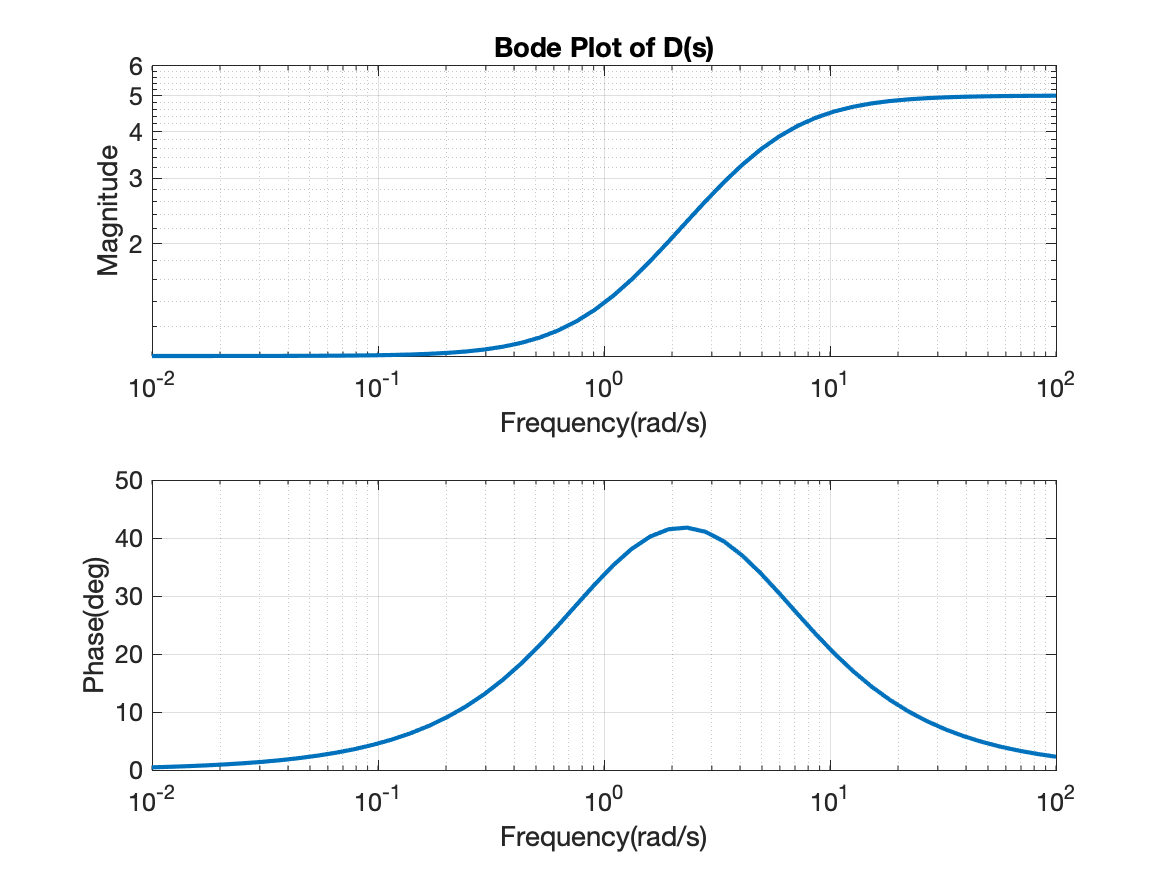
\includegraphics[width = 0.6\textwidth]{pic/0.png}
% \end{figure}

% $$
% A = 
% \left [
% \begin{matrix}
%    -1 & 0 \\
%    1 & 0
% \end{matrix}
% \right ],\ \ \
% $$

% \begin{equation*}
% f_U(u) = 
% \left\{
% \begin{aligned}
% & 0 &&,\ u<-5\\
% & \frac{u+5}{8} &&,\ -5\leq u < -3\\
% \end{aligned}
% \right.
% \end{equation*}

\section{Problem 1}
\subsection{Part A}
The state equation and the output equation:
\begin{equation*}
\left
\begin{aligned}
& \dot{x}_1 = -5 x_1 - 4x_3 + u\\
& \dot{x}_2 = x_1\\
& \dot{x}_3 = x_2\\
& y = 100x_3
\end{aligned}
\right.
\end{equation*}
So the control matrices are:
$$
A =  \left [
\begin{matrix}
   -5 & -4 & 0 \\
   1 & 0 & 0 \\
   0 & 1 & 0 \\
\end{matrix}
\right ], \ \ \ 
$$





\end{document}